\documentclass[tikz,border=10pt]{standalone}

\usepackage{xcolor}
\usetikzlibrary{arrows.meta, positioning}

\definecolor{paperGreen}{RGB}{34,125,92}
\definecolor{paperSoft}{RGB}{246,248,250}
\definecolor{paperLine}{RGB}{80,92,110}

\begin{document}
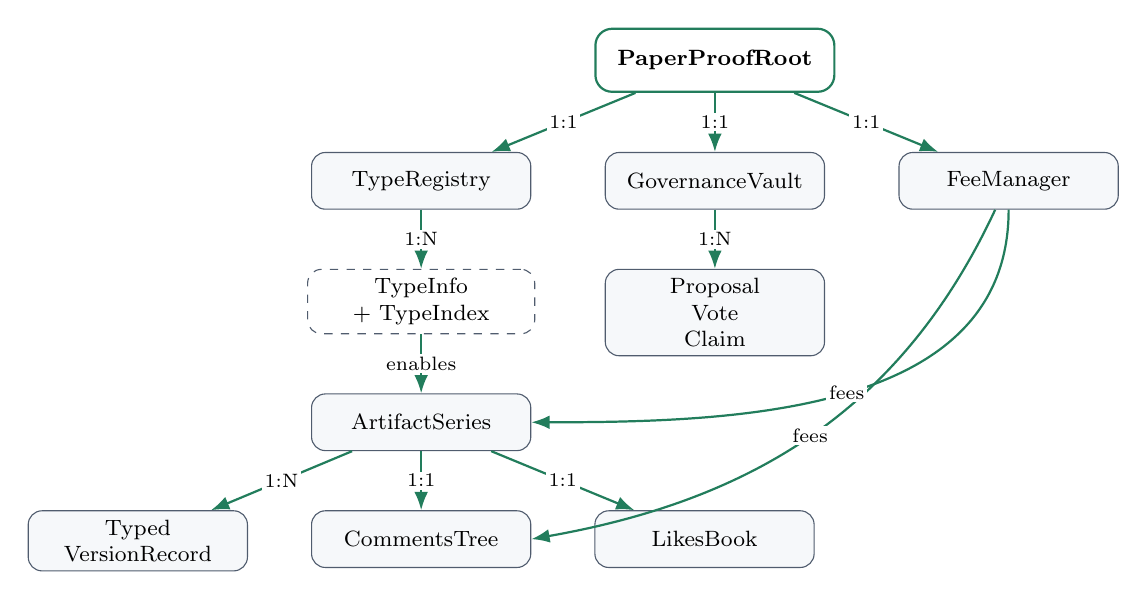
\begin{tikzpicture}[
    obj/.style={draw=paperLine, rounded corners=5pt, fill=paperSoft, minimum height=0.72cm, align=center, font=\footnotesize, text width=2.55cm},
    root/.style={draw=paperGreen, thick, rounded corners=6pt, fill=white, minimum height=0.8cm, align=center, font=\footnotesize\bfseries, text width=2.8cm},
    logical/.style={draw=paperLine, dashed, rounded corners=5pt, fill=white, minimum height=0.72cm, align=center, font=\footnotesize, text width=2.65cm},
    arrow/.style={-Latex, thick, draw=paperGreen},
    rel/.style={font=\scriptsize, fill=white, inner sep=1pt},
    node distance=0.75cm and 0.8cm
]
    \node[root] (root) {PaperProofRoot};
    \node[obj, below left=of root] (registry) {TypeRegistry};
    \node[obj, below=of root] (vault) {GovernanceVault};
    \node[obj, below right=of root] (fee) {FeeManager};
    \node[logical, below=of registry] (typeinfo) {TypeInfo\\+ TypeIndex};
    \node[obj, below=of typeinfo] (series) {ArtifactSeries};
    \node[obj, below left=of series] (version) {Typed\\VersionRecord};
    \node[obj, below=of series] (comments) {CommentsTree};
    \node[obj, below right=of series] (likes) {LikesBook};
    \node[obj, below=of vault] (proposal) {Proposal\\Vote\\Claim};

    \draw[arrow] (root) -- node[rel] {1:1} (registry);
    \draw[arrow] (root) -- node[rel] {1:1} (vault);
    \draw[arrow] (root) -- node[rel] {1:1} (fee);
    \draw[arrow] (registry) -- node[rel] {1:N} (typeinfo);
    \draw[arrow] (typeinfo) -- node[rel] {enables} (series);
    \draw[arrow] (series) -- node[rel] {1:N} (version);
    \draw[arrow] (series) -- node[rel] {1:1} (comments);
    \draw[arrow] (series) -- node[rel] {1:1} (likes);
    \draw[arrow] (vault) -- node[rel] {1:N} (proposal);
    \draw[arrow] (fee) to[out=-115,in=10] node[rel] {fees} (comments.east);
    \draw[arrow] (fee) to[out=-90,in=0] node[rel] {fees} (series.east);
\end{tikzpicture}
\end{document}
